\section{Introduction}\label{sec:intro}

DNSSEC is not a new technology; it has been in development since 1995, with the
first RFC published in 1997.\cite{dnssecHistory} Unfortunately, deployment 
has been slow but incremental due to, among other reasons, significant 
infrastructure investments needed to handle the overhead costs
required to verify DNSSEC responses.

DNSSEC requires verification of a certificate signature chain in order to 
maintain security. There are fourfold costs. First are calculating the 
signatures. Fortunately, this cost is getting cheaper due to processor 
improvements and is not the focus of this paper. Second are the additional DNS 
query costs. In order to verify signatures, DNS resolvers must request 
additional signature-related DNS records from various servers on the certificate
chain.
Third are the additional bandwidth costs. There are additional DNSSEC-specific 
records contributing, but the extra queries are a bulk of the extra bandwidth 
needs.
In one study, these two costs were estimated such that 
resolvers would need to be sized to ``handle 10 times the query volume ... and a
total response traffic volume of 100 times greater.''\cite{huston2013} 
Finally, there are the latency costs for end hosts as the verification 
activities take  non-trivial time.

These costs are significant, especially regarding equipment provisioning. We 
seek to reduce these costs by relying on an \emph{outside source of trust} in
place of signature verification. 
By using a different way of finding trust between DNSSEC-enabled resolvers, we 
can cut down on the amount of PKI verifications and further queries that are 
necessary for traditional DNSSEC. 

\begin{figure}
  \centering
  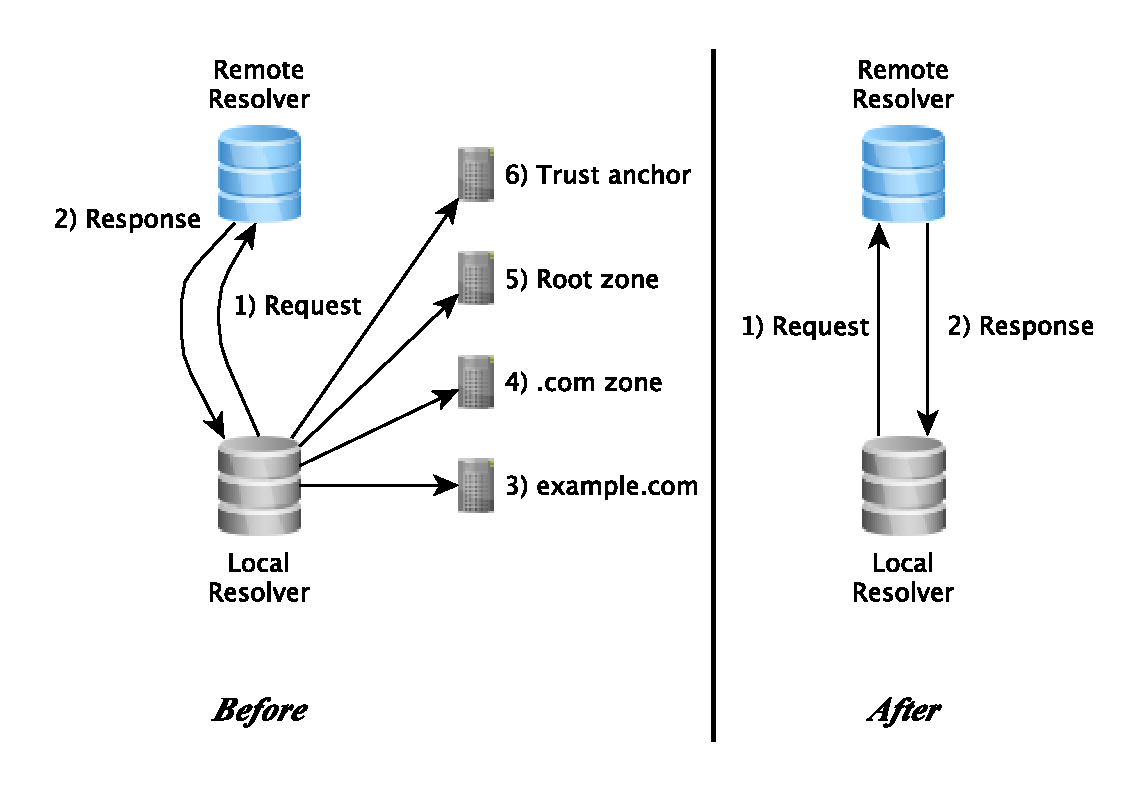
\includegraphics[width=1.0\columnwidth]{figures/before-and-after}
  \caption{Before, to verify the certificate chain that DNSSEC relies upon, many further requests for RRSIG and DS resources are necessary to verify signatures. With our proposal, there is a long-lived, mutually authenticated TLS connection between both resolvers that the requests and responses travel across. If the local resolver knows who is at the other end of the connection, and it trusts that the remote resolver has verified signatures, the local resolver should not need to verify the same signatures itself.}
  \label{fig:before-and-after}
\end{figure}


%\begin{figure}
%  \begin{minipage}{\textwidth}
%  \begin{minipage}{\columnwidth}
%    \begin{subfigure}{.5\columnwidth}
%      \centering
%      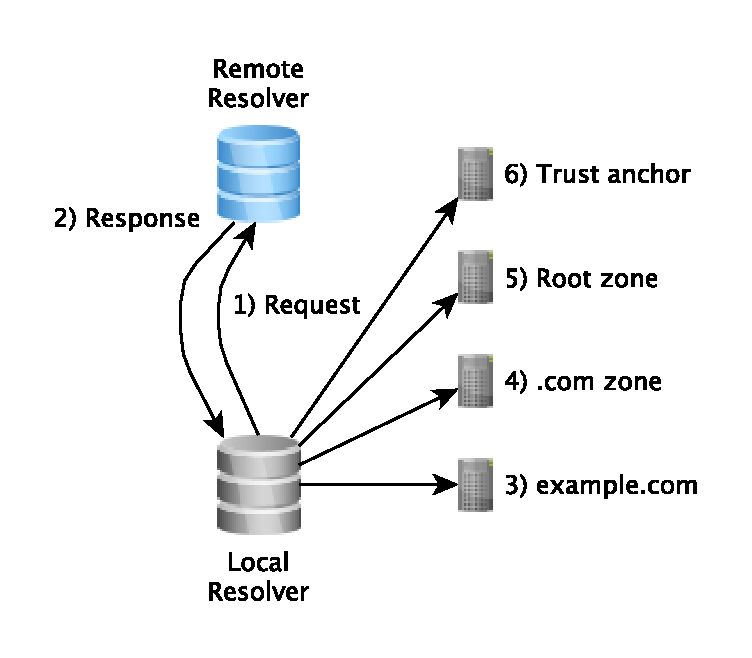
\includegraphics[width=1.0\columnwidth]{figures/before}
%      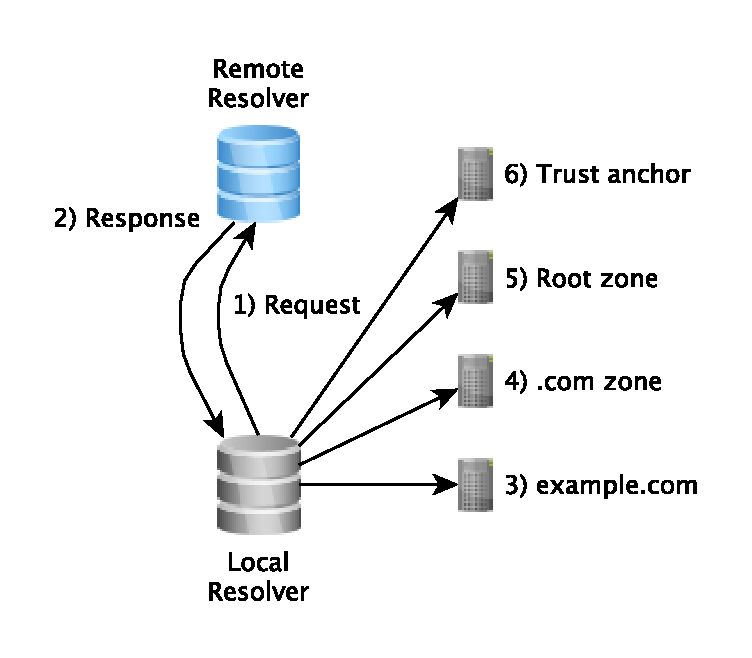
\includegraphics[width=.8\columnwidth]{figures/before}
%      \caption{\textbf{Before}}
%      \label{fig:before}
%    \end{subfigure}
%    \begin{subfigure}{.5\columnwidth}
%      \centering
%      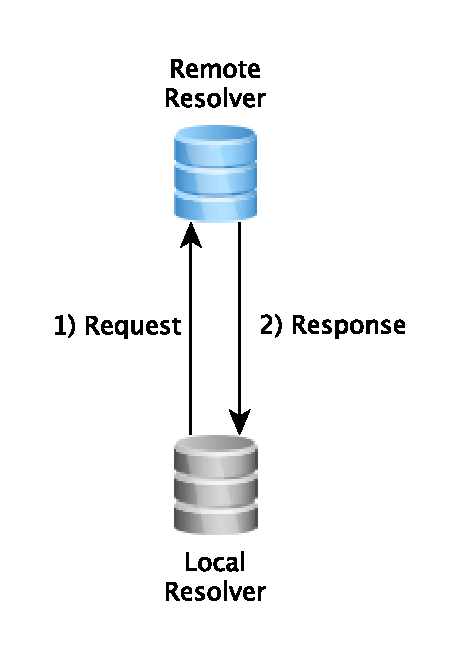
\includegraphics[width=.6\columnwidth]{figures/after}
%      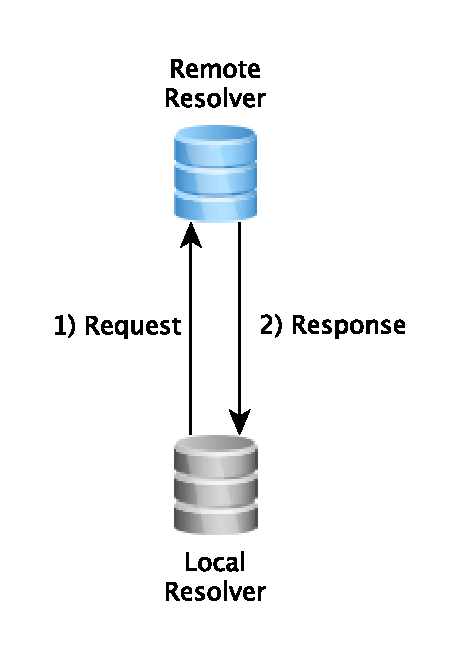
\includegraphics[width=.6\columnwidth]{figures/after}
%      \caption{\textbf{After}}
%      \label{fig:after}
%    \end{subfigure}
%    \caption{For DNSSEC, verifying the DNSSEC signature chain requires many requests to many different remote servers. With our proposal, there is no additional verification strictly necessary.}
%    \label{fig:before-and-after}
%  \end{minipage}
%\end{figure}  




